\documentclass{article}
\usepackage{polski}
\usepackage[utf8]{inputenc}
\usepackage[OT4]{fontenc}
\usepackage{graphicx,color}
\usepackage{url}
\usepackage[pdftex,hyperfootnotes=false,pdfborder={0 0 0}]{hyperref}
\usepackage{float}

\begin{document}
\thispagestyle{empty} %bez numeru strony

\begin{center}
{\large{Sprawozdanie z laboratorium:\\
Komunikacja człowiek–komputer}}

\vspace{3ex}

Przetwarzanie obrazu — aplikacja

\vspace{3ex}
{\footnotesize\today}

\end{center}


\vspace{10ex}

Prowadzący: dr hab.~inż. Maciej Komosiński

\vspace{5ex}

Autorzy:
\begin{tabular}{lllr}
\textbf{Sebastian Firlik} & inf122485 & sebastian.firlik@student.put.poznan.pl \\
\textbf{Adam Pioterek} & inf122446 & adam.pioterek@student.put.poznan.pl \\
\end{tabular}

\vspace{5ex}

Zajęcia czwartkowe, 15:10.

\vspace{35ex}

\noindent Oświadczam/y, że niniejsze sprawozdanie zostało przygotowane wyłącznie przez powyższych autora/ów,
a wszystkie elementy pochodzące z innych źródeł zostały odpowiednio zaznaczone i~są cytowane w bibliografii.  

\newpage



\section*{Udział autorów}
\begin{itemize}
\item Sebastian Firlik -- stworzenie zbioru danych, implementacja funkcji liczącej atrybuty warunkowe, stworzenie i nauczenie klasyfikatora, wizualizacja drzewa decyzyjnego
\item Adam Pioterek — implementacja wykrywania samochodów na obrazie oraz ekstrahowania wielokątów zawierających samochody.
\end{itemize}

\section{Filtry i funkcje}
Do rozwiązania naszego zadania użyliśmy biblioteki skimage do przetwarzania obrazów, sklearn w celu pozyskania drzewa decyzyjnego, czyli naszego klasyfikatora, scipy do funkcji wykrywającej otoczkę wypukłą, numpy do manipulowania tablicami.

Do wykonania zadania wykorzystane zostały następujące filtry:
\begin{description}
\item[gaussian] — przeprowadza rozmycie Gaussa;\\
na wejściu otrzymuje zdjęcie w odcieniach szarości (macierz 2D) i odchylenie standardowe, na wyjściu daje macierz 2D – przefiltrowane zdjęcie.
Jego zadaniem jest rozmycie obrazu i tym samym pozbycie się niepotrzebnych i zaniedbywalnych szczegółów  a także szumów z naszego obrazu. Parametrem rozmycia Gaussa jest odchylenie standardowe $\sigma$ rozkładu normalnego. Im większe ono jest tym bardziej rozmyty jest obraz. W naszym programie $\sigma = 5$. 
\item[scharr] — odmiana filtru Sobela ze specjalnie dobranymi operatorami;\\
na wejściu funkcji musimy podać macierz z obrazem, gdzie w każdej komórce musi być jedna wartość (obraz w skali szarości, w jednym określonym kolorze). Opcjonalnie możemy podać maskę filtrowania. Wyjściem z funkcji jest przetransformowany obraz. Wybraliśmy filtr Scharra, ponieważ jest najbardziej niewrażliwy na rotację spośród innych dostępnych w bibliotece skimage (Sobel, Prewitt, Canny).
\item[dylatacja] — morfologiczna dylatacja, która powiększa jasne rejony na rzecz ciemnych;
na wejściu otrzymuje zdjęcie w odcieniach szarości (macierz 2D), na wyjściu daje macierz 2D.
\item[erozja] — morfologiczna erozja, która powiększa ciemne rejony na rzecz jasnych;
na wejściu otrzymuje zdjęcie w odcieniach szarości (macierz 2D), na wyjściu daje macierz 2D.
\end{description}
oraz funkcje:
\begin{description}
\item[threshold\_otsu] — progowanie Otsu, redukujące szarość do binarnego podziału na biel i czerń;\\
dzięki temu progowaniu otrzymaliśmy obraz biało-czarny, bez żadnych dodatkowych szarości. W ten sposób łatwiej nam było pozbyć się tła z obrazka.
\item[moments\_hu] — momenty Hu;\\
na wejściu otrzymuje znormalizowane momenty centralne, na wyjściu daje listę momentów Hu.
\item[ConvexHull] — otoczka wypukła;\\
na wejściu otrzymuje zbiór punktów, na wyjściu zwraca indeksy punktów należących do otoczki.
\end{description}

By obliczyć momenty Hu musieliśmy wcześniej obliczyć zwyczajne momenty obrazka, następnie momenty centralne, później znormalizowane momenty centralne i dopiero wtedy mogliśmy przystąpić do obliczenia momentów Hu, które posłużyły nam jako cechy naszego obrazka.

Wyjściem z ostatniej funkcji -- ConvexHull -- jest otoczka, którą przekształcamy w listę wierzchołków. Stanowią one wierzchołki wypukłego konturu samochodu. Następnie uruchamiamy naszą funkcję feature\_detection, której zadaniem jest uzyskać z danego na wejściu rozmiaru obrazka i konturu samochodu nasze cechy, opisane dalej. Wynik działania naszych filtrów i funkcji ConvexHull możemy zobaczyć na poniższym obrazku:

\begin{figure}[H]
\begin{center}
\includegraphics[width=1\textwidth]{./images/advanced.pdf}
\end{center}
\caption{Wykrywanie otoczki wypukłej na kilku samochodach}
\label{fig: wykres2}
\end{figure}

Na końcu zapisujemy cechy, związane z każdym z obrazków do pliku CSV, co pozwala nam utworzyć w przyszłości zbiór uczący i testowy naszego klasyfikatora.

W pliku classify.py znajduje się skrypt, którego celem jest stworzenie drzewa decyzyjnego (CART), nauczenie go wzorców na podstawie naszych losowo wybranych danych treningowych, a następnie przetestowanie przykładów, które nie zostały użyte do procesu uczenia. Po zakończeniu działania programu otrzymujemy wizualizację drzewa decyzyjnego z podziałami na różnych atrybutach
 
\section{Cel eksperymentu}
Celem eksperymentu było stworzenie systemu rozpoznającego na zdjęciach samochody i kategoryzującego rozpoznane samochody jako sedan, suv lub van. W zamierzeniu nasza aplikacja mogłaby posłużyć jako część składowa większego systemu, który wspomagałby proces wybierania kategorii na serwisach ogłoszeniowych przez użytkowników już na etapie tworzenia ogłoszenia, kiedy dodajemy zdjęcia, prezentujące nasz samochód.
\section{Dane do eksperymentu}
Nasze zdjęcia uzyskaliśmy poprzez wpisywanie fraz Suv, Sedan, Van w wyszukiwarkę Google Grafika. Często dodawaliśmy do typu samochodu również jego markę, by zróżnorodnić nasz zbiór zdjęć. Końcowo zebraliśmy 75 zdjęć, na których widnieją samochody, ich cienie, napisy i tło, najczęściej w postaci gradientu lub przezroczystości w przypadku obrazków w formacie .png.
\begin{figure}[H]
\begin{center}
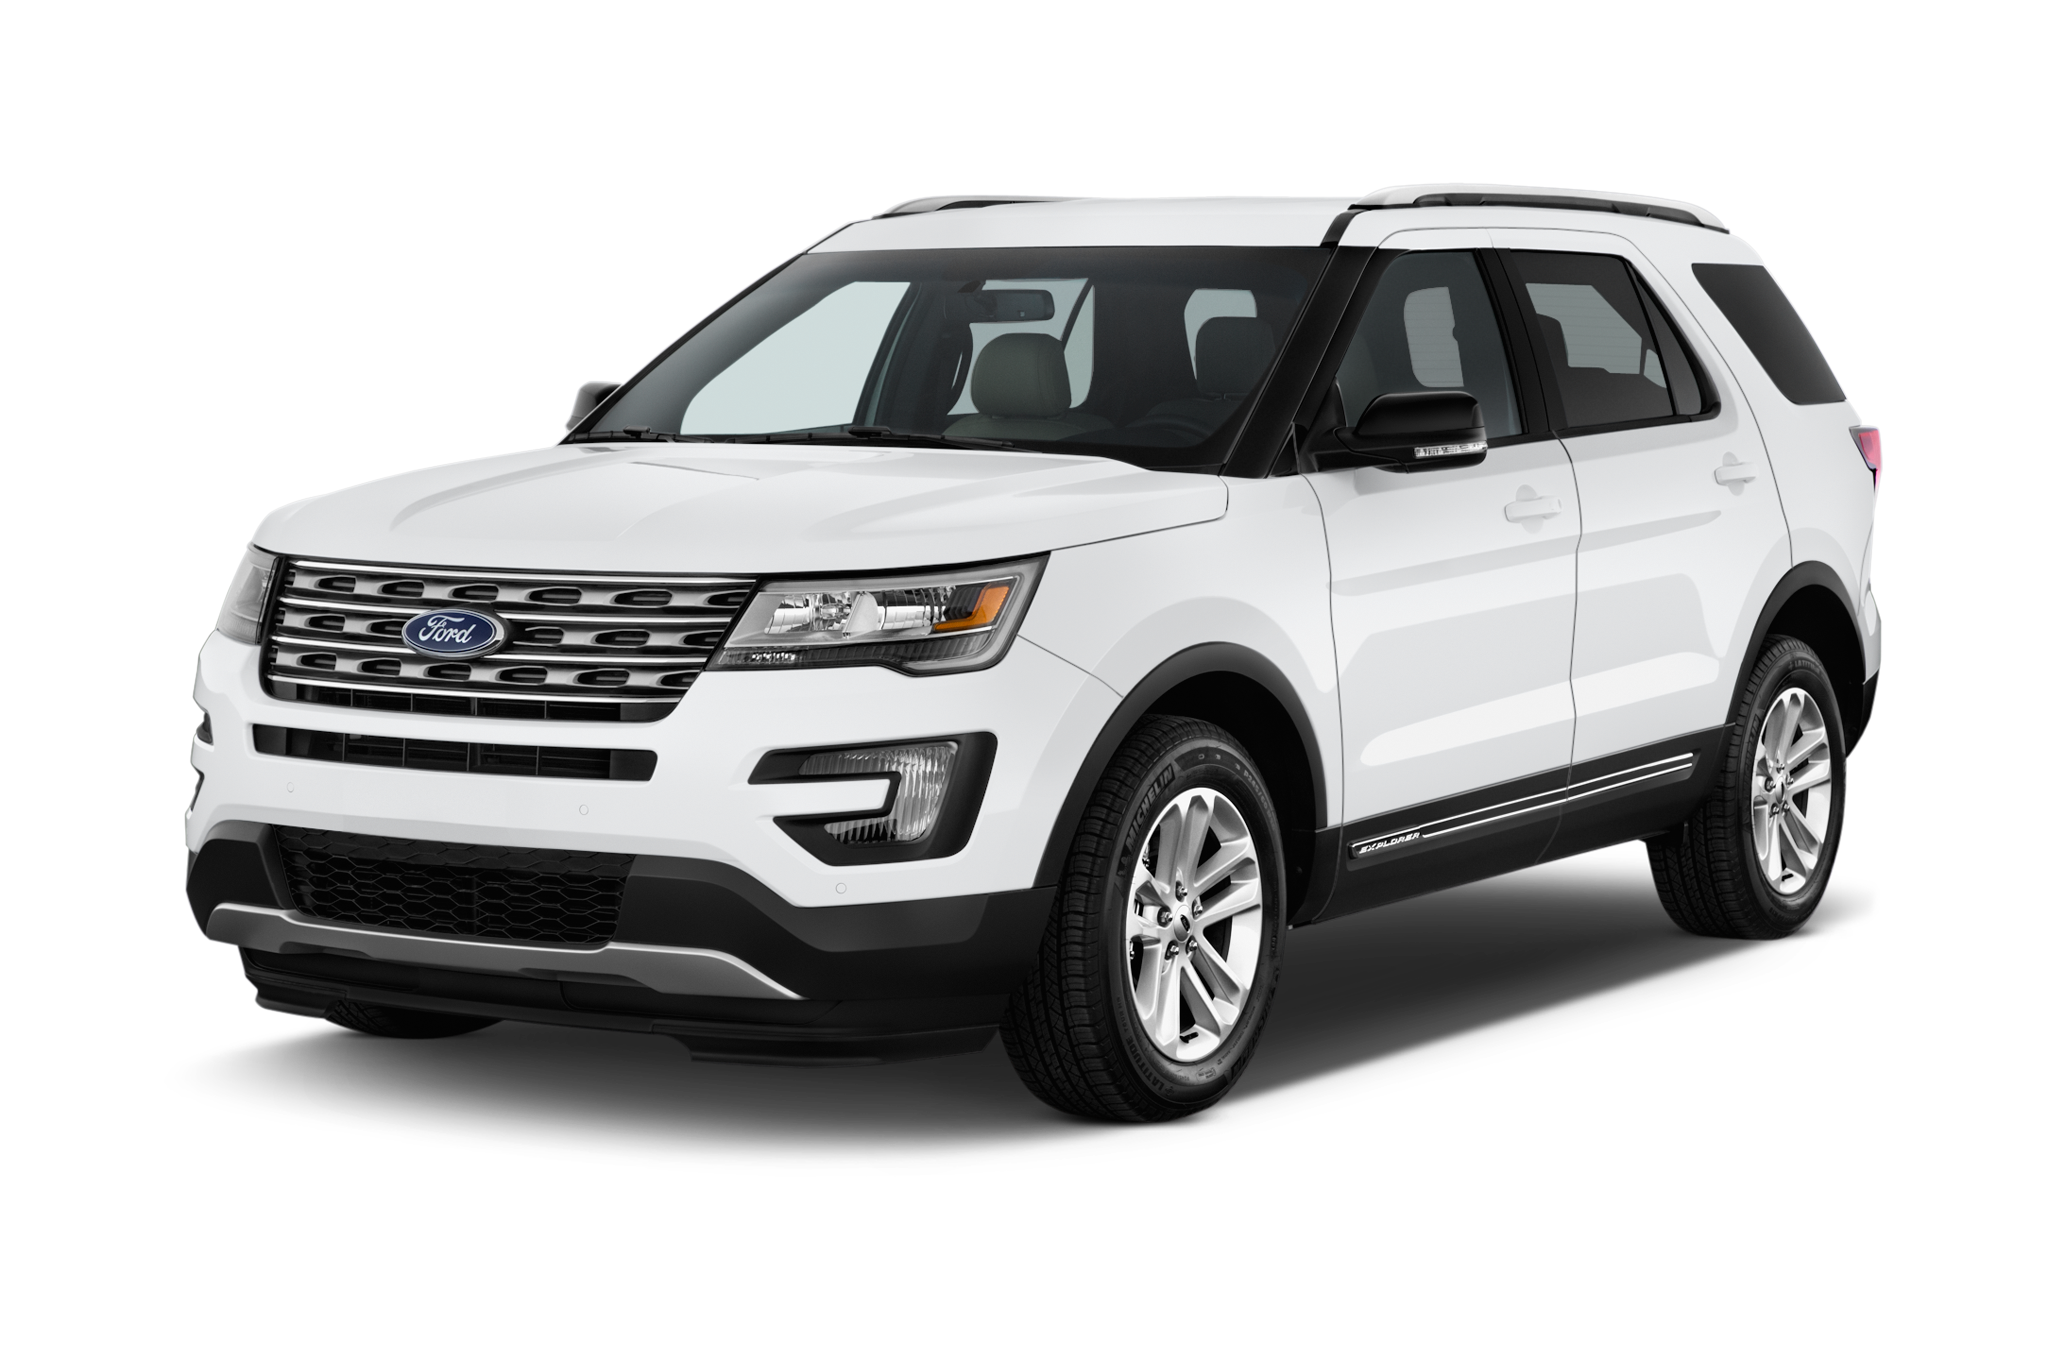
\includegraphics[width=1\textwidth]{../imgs_easy/suv_07.png}
\end{center}
\caption{Jeden z samochodów typu SUV}
\label{fig: wykres1}
\end{figure}

\begin{figure}[H]
\begin{center}
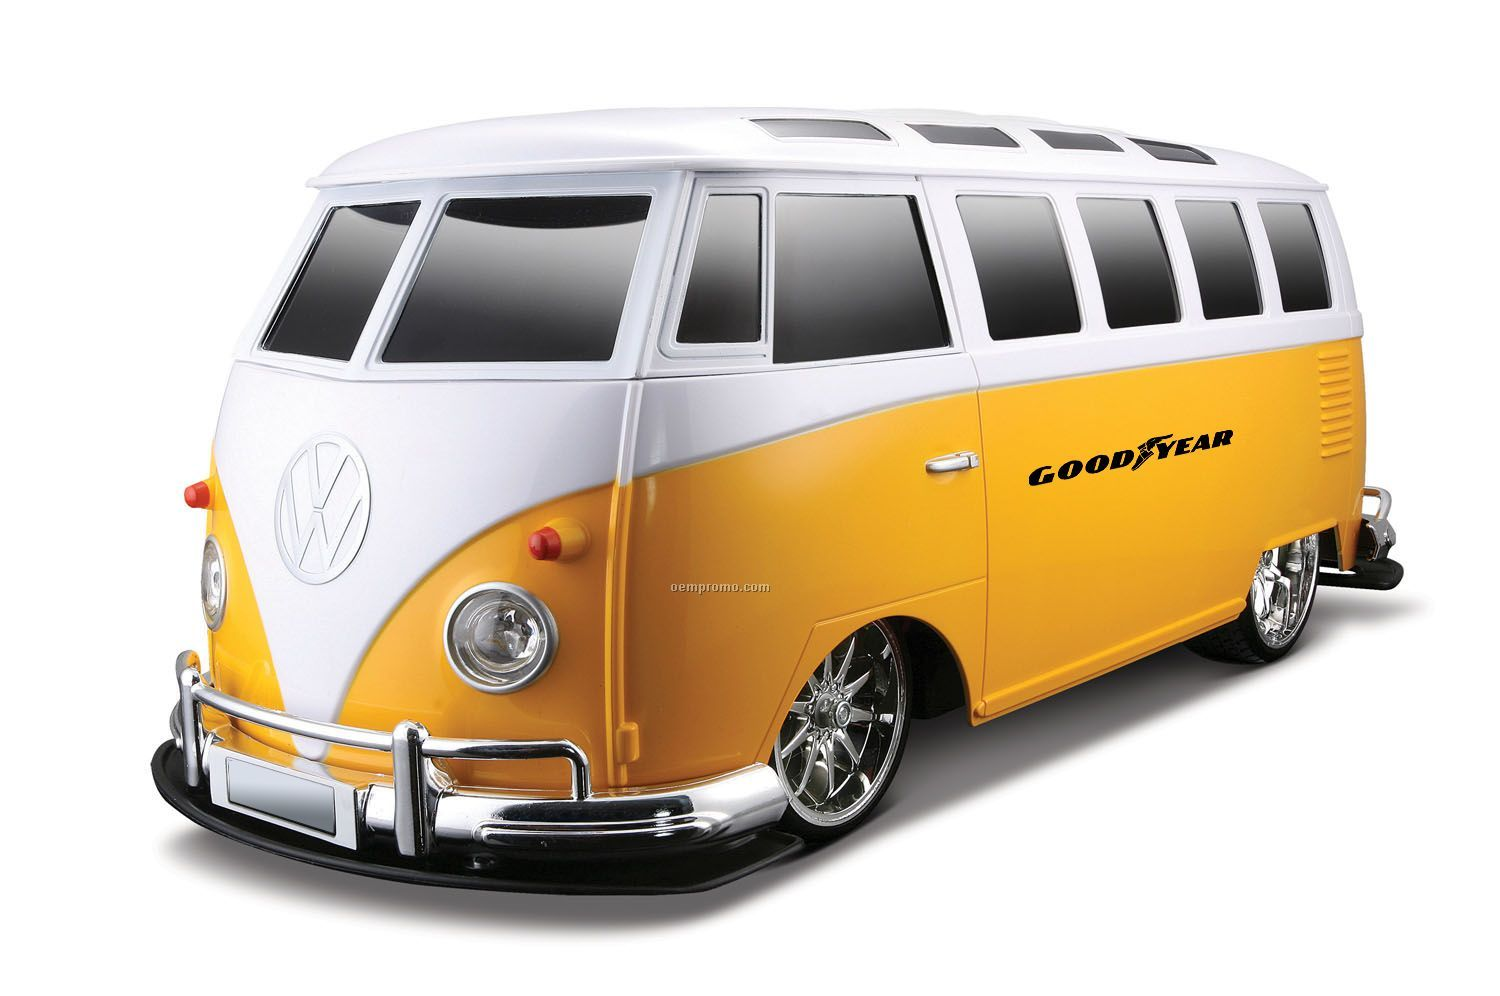
\includegraphics[width=1\textwidth]{../imgs_easy/van_19.jpg}
\end{center}
\caption{Samochód typu Van}
\label{fig: wykres2}
\end{figure}

\begin{figure}[H]
\begin{center}
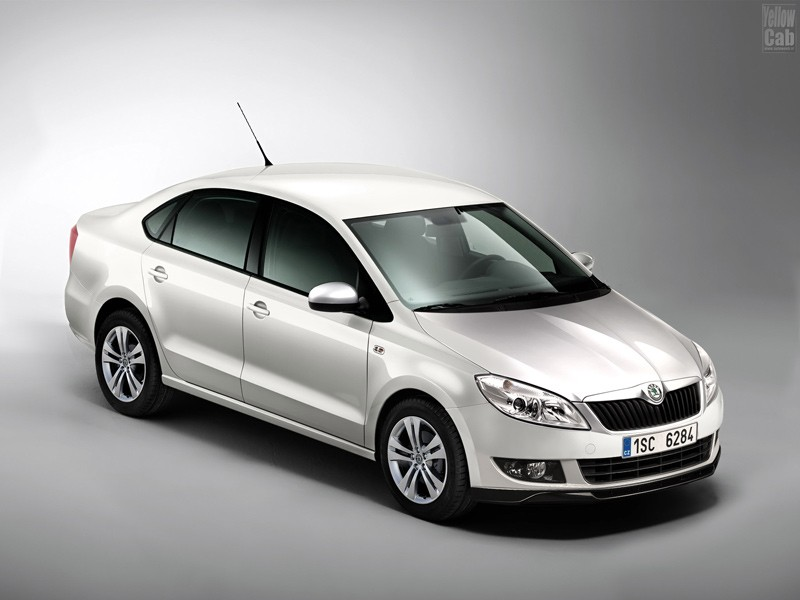
\includegraphics[width=1\textwidth]{../imgs_easy/sedan_22.jpg}
\end{center}
\caption{Samochód typu Sedan}
\label{fig: wykres3}
\end{figure}
\section{Rozwiązanie i efektywność}
Nasz program generował 12 atrybutów warunkowych i 1 atrybut decyzyjny dla każdego obrazka. Atrybut decyzyjny miał jedną z trzech wartości ze zbioru ${d, s, v}$, odpowiednio dla samochodów typu sedan, suv i van. Natomiast pośród atrybutów warunkowych możemy wyróżnić:
\begin{enumerate}
\item Siedem momentów Hu
\item Stosunek obwodu otoczki wypukłej samochodu do jej pola
\item Znormalizowana wysokość konturu -- osiągnęliśmy to dzięki podzieleniu różnicy maksimum i minimum współrzędnych \textit{y} przez wysokość całego obrazka w pikselach.
\item Stosunek wysokości samochodu do jego długości
\item Stosunek pola powierzchni samochodu do pola całego obrazka
\item Liczba wierzchołków otoczki wypukłej samochodu -- wklęsłe wierzchołki przy oponach samochodów zostały usunięte w procesie tworzenia otoczki, jednak nie wpływa to negatywnie na ważność tej cechy, ponieważ każdy samochód ma te wierzchołki, więc możemy je od każdego przykładu odjąć.
\end{enumerate}

Atrybuty te zapisywaliśmy dla każdego obrazu w osobnej linii do pliku .csv. Dzięki temu stworzyliśmy sobie plik, w którym mieliśmy pełne dane o każdym z samochodów. Do klasyfikacji postanowiliśmy użyć drzewa decyzyjnego CART (Classification And Regression Tree) z pakietu sklearn. Utworzyliśmy obiekt klasy DecisionTreeClasifier, a następnie wytrenowaliśmy go na danych treningowych -- pięćdziesięciu losowych obiektach z pliku .csv. Oddzieliśmy atrybuty warunkowe od decyzyjnego, a następnie takie listy list daliśmy jako atrybuty metody \textit{fit} drzewa decyzyjnego. Wybraliśmy drzewo decyzyjne na nasz klasyfikator, ponieważ jest ono łatwe w wizualizacji i interpretacji - otrzymujemy liniowe podziały przestrzeni atrybutów warunkowych na konkretnych atrybutach i w liściach otrzymujemy już konkretny przydział do klas na podstawie poprzednich przydziałów, od korzenia drzewa, do danego liścia.

Wykorzystaliśmy również pole feature\_importances\_ z obiektu drzewa decyzyjnego, które to pole zawierało listę ważności poszczególnych atrybutów, które wygenerowaliśmy. Warto odnotować, że każdy atrybut, który sami wymyśliliśmy i wygenerowaliśmy miał ważność większą od zera, natomiast niektóre spośród siedmiu momentów Hu miały tę wartość równą zero.

Stwierdziliśmy, że podziały przestrzeni, które generuje drzewo są wystarczające dla naszego problemu, mimo tego, że nie zbadaliśmy rozkładu w przestrzeni naszych przykładów. Pozostaliśmy głównie przy zadaniu analizy obrazów, nie zagłębiając się zbytnio w kwestie związane z uczeniem maszynowym, co jednak pozwoliło nam uzyskać przyzwoite rezultaty. Przykładowa macierz pomyłek, wygenerowana z wyników naszej klasyfikacji jest przedstawiona poniżej:
\begin{table}[h]
\begin{center}
\begin{tabular}{|c||c|c|c|}
\hline
Real/Pred & Sedan & SUV & Van\\
\hline
Sedan & 3 & 0 & 0\\
\hline
SUV & 2 & 4 & 0\\
\hline
Van & 2 & 3 & 1\\
\hline
\end{tabular}
\end{center}
\caption{Przykładowa macierz konfuzji dla naszego problemu}
\end{table}

Kolejne wiersze powyższej tabeli to klasy prawdziwe danego obiektu, natomiast kolumny to klasy przewidziane przez nasz program. Z takiej macierzy pomyłek możemy obliczyć na przykład trafność klasyfikacji:

\begin{equation}
Accuracy = \frac{3 + 4 + 1}{15} = \frac{8}{15} = 0,5(3)
\end{equation}

Referencyjną wartością naszej trafności jest przypadek, gdy wszystkie przykłady "z góry" umieścimy w jednej, najliczniejszej klasie. U nas mamy trzy równoliczne klasy, więc minimalnie powinniśmy uzyskać trafność klasyfikacji na poziomie $33\%$. W naszym przypadku trafność wynosi ponad $50\%$, więc nasze znalezione cechy są ważne w rozwiązywaniu tego problemu klasyfikacji. Oczywiście zależnie od wylosowanych do zbioru treningowego przykładów, trafność może się różnić, jednak podana wartość jest wartością często się powtarzającą, bliską średniej. Zdarzały się przypadki, w których nawet 11 na 15 samochodów było dobrze klasyfikowanych. 

\begin{figure}[H]
\begin{center}
\includegraphics[width=1\textwidth]{./images/cars.pdf}
\end{center}
\caption{Przykładowa wizualizacja naszego drzewa decyzyjnego}
\label{fig: wykres3}
\end{figure}

Na powyższym rysunku widzimy jedno z możliwych drzew decyzyjnych, wygenerowanych dla pewnej instancji naszego problemu. Na samej górze każdego wierzchołka nie będącego liściem zauważamy jedną z naszych cech i nierówność. To sygnalizuje, że w lewym poddrzewie będą się znajdować wszystkie przykłady spełniające tę nierówność, a po prawej te niespełniające nierówności. Współczynnik gini jest jedną z metod okreslenia ważności podziału, samples mówi nam, jak wiele przykładów znajduje się w danym wierzchołku. Class natomiast to dominująca w danym wierzchołku, lub wybrana w liściu klasa przykładów.

\section{Podsumowanie}
Podstawowy cel naszej aplikacji został osiągnięty. Poprawiliśmy jakość klasyfikacji dość znacznie ponad referencyjne $33\%$, z czego możemy wnioskować, że nasze cechy są ważne w naszym problemie i poszliśmy dobrą drogą. Użyliśmy różnych filtrów i sposóbów na wyłuskanie z obrazu konturu samochodu, a dokładniej otoczki wypukłej samochodu. Nie wyszło nam to idealnie w stu procentach, ponieważ różne szumy na obrazie, lub blisko siebie identyczne kolory czasami zakłócały proces wykrywania konturu, jednak końcowo efekt wygląda całkiem nieźle. 

Nauczyliśmy się podstaw kontrukcji systemu uczącego się i interpretacji uzyskanych wyników, a także tworzenia zbiorów danych, które są różnorodne i mają wiele interesujących cech podobnych wewnątrz każdej z klas, a nie występujących pomiędzy klasami. Zwizualizowaliśmy macierz konfuzji dla naszego problemu, a także obliczyliśmy trafność klasyfikacji dla wielu różnych instancji naszego problemu.

Niestety im więcej szumu, cieni, napisów na zdjęciu, tym trudniej jest nam uzyskać ładny jeden kontur. Kolejną przeszkodą w prawidłowym rozpoznaniu typu samochodu na zdjęciu jest sytuacja, gdy samochód jest obrócony tyłem, lub widzimy go dokładnie od przodu -- wtedy pewne cechy tracą swoją pierwotną ważność, ponieważ patrząc na samochód od przodu nie widzimy jego długości, jedynie szerokość i wysokość, a jedną z cech jest stosunek wysokości samochodu do jego długości.

Podsumowując, nasza aplikacja spełnia swoją rolę, lecz wiele rzeczy jest do poprawy, by działała idealnie. Zaletą naszego rozwiązania jest fakt wykorzystania prostych filtrów na obrazie wejściowym i proste cechy, które znaleźliśmy i obliczyliśmy.

\end{document}